%%=============================================================================
%% Methodologie
%%=============================================================================

\lstset{
	basicstyle=\ttfamily,
	columns=fullflexible,
	frame=single,
	breaklines=true
}

\chapter{\IfLanguageName{dutch}{Proof of Concept}{Proof of Concept}}
\label{ch:proofofconcept}

\section{Setting up a new Drupal 9 site}

Creating a new Drupal 9 site with the standard Drupal 9 profile on a local server environment is fairly simple. Some different steps are involved depending on the Operating System, but overall the workflow goes like this: 
\begin{itemize}
	\item Create a local environment using an AMP (Apache HTTP server, MySQL relational database, PHP programming language) stack. On the most popular OSs, Linux, Windows and MacOS, packages are available that include all of these technologies. These allow for a smooth and simple process of installing a local environment.
	\item Installing Drupal. The latest release of Drupal can always be found on the \url{https://drupal.org} site.
\end{itemize}

\subsection{Setting up a local environment}

In this proof of concept, MAMP will be used to create a local server environment. MAMP is a tool for MacOS that allows you to easily set up such an environment. The folder structure provided by MAMP should look like in figure \ref{fig:MAMP_Structure}. The most important directory here will be the htdocs directory. This folder will house all the Drupal files. 

\begin{figure}
	\centering
	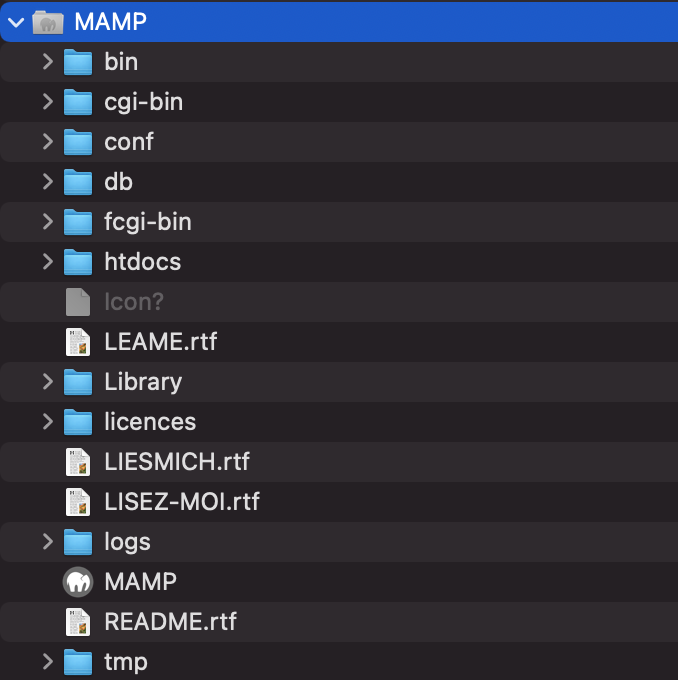
\includegraphics[width=10cm]{./img/MAMP_Structure.png}
	\caption[MAMP folder structure]{The folder structure provided by MAMP}
	\label{fig:MAMP_Structure}
\end{figure}

The files for Drupal 9 can be found on \url{https://drupal.org/download}. When these have been downloaded, they need to be put into the \emph{htdocs} folder inside of MAMP. When starting up MAMP, a graphical interface is launched inside the browser, which has the option to go to your website on the following local address: http://localhost:8888. After that, the actual installation of Drupal can begin.

\begin{figure}
	\centering
	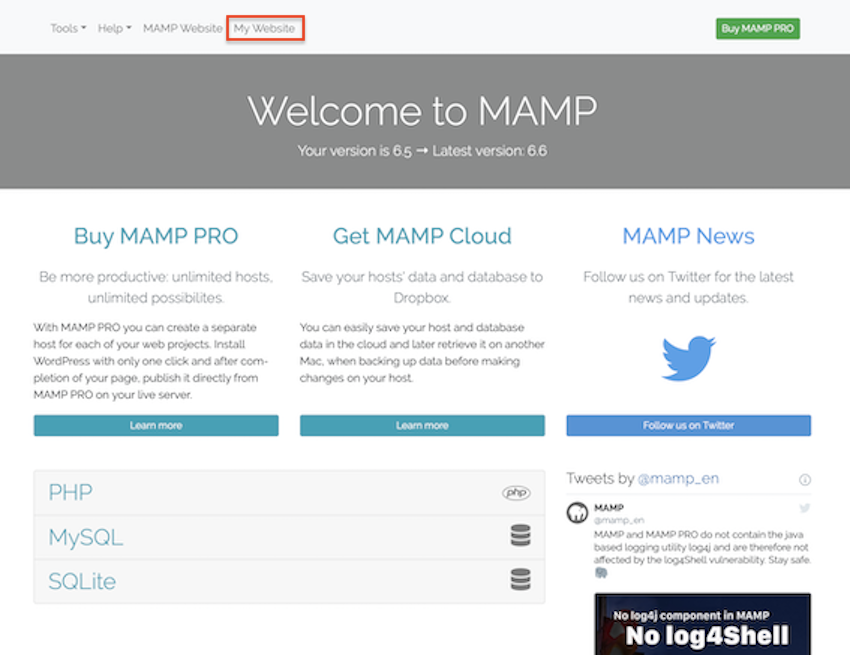
\includegraphics[width=10cm]{./img/MAMP_Web.png}
	\caption[MAMP interface]{The graphical interface provided by MAMP}
	\label{fig:MAMP_Web}
\end{figure}

\subsection{Drupal 9 installation}

Drupal 9 can be installed in two ways: by using drush, or by using the graphical user interface. 

Drush is, according to \textcite{Tomlinson2015}, \emph{"a command line tool that greatly simplifies the tasks of building and administering a Drupal website."} Drush allows you to perform specific tasks related to your Drupal website, one of which is installing the website.

For this proof of concept, the Drupal 9 graphical user interface will be used, as it is still the most straight forward way of installing Drupal. When using this interface, Drupal 9 will prompt you through a few steps:

\begin{enumerate}
	\item Choosing the default installation language.
	\item Choosing an installation profile. Drupal 9 core comes with two default profiles that can be chosen. Firstly there is the standard profile. This profile comes with commonly used features already pre-configured. Secondly, the minimal profile is used to build a completely custom site without pre-configured functionality. There is also a demo profile included, which comes with some content already in the system. This can be used for testing out the possibilities of Drupal 9. For this research the standard profile will be used.
	\item Setting up the database. In most cases, this step will be configured automatically by the installer. In some rare occasions though, there might be an issue that needs to be resolved by the site administrator.
	\item Install site. This step will automatically install the Drupal 9 site on your system. As with the previous step, there might be some issues that need to be resolved before the installation can be completed.
	\item Configuration of the site. In this step, you will be asked to configure some important settings. The site information, including the site name and e-mail address, need to be filled in, and you will need to configure an administration account for your website. The name of this account is usually \emph{admin}. After that, regional settings and update information need to be configured.
	\begin{figure}
		\centering
		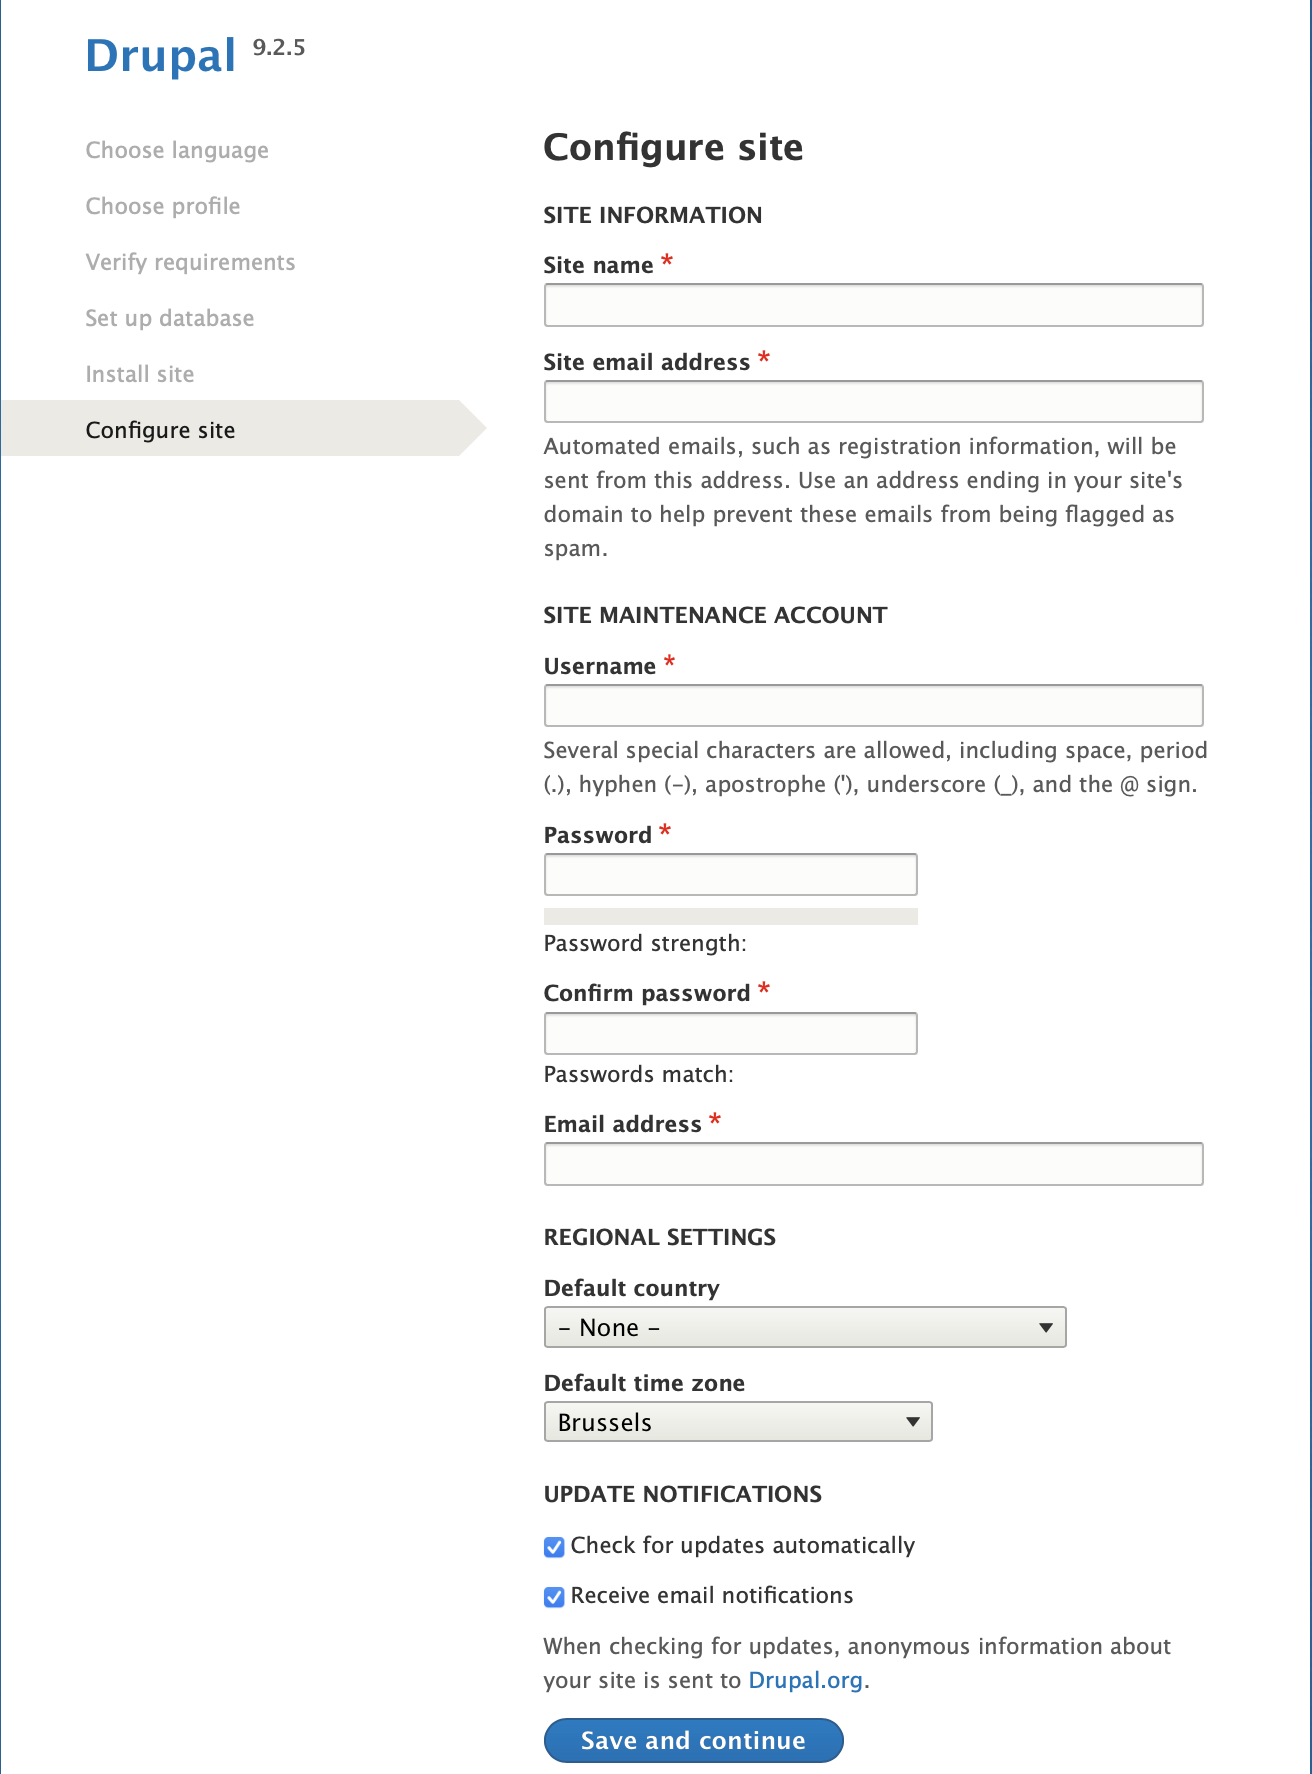
\includegraphics[width=10cm]{./img/Install_Config.png}
		\caption[Configuring Drupal 9]{Configuring your Drupal 9 site}
	\end{figure}
\end{enumerate}

When all these steps are completed, a new Drupal 9 site is ready for use. Before getting started with adding content to the site, there are a few optional things to do to improve the user experience.

\subsubsection{Installing modules and themes}

Installing modules in Drupal 9 is a fairly simple process. Modules that are included in Drupal 9 core can be easily enabeled through the user interface by going to \url{http://localhost:8888/admin/modules}. Contributed modules, available on \url{https://www.drupal.org} are a little trickier. The best way to install these is via the use of \emph{Composer}. As mentioned in section \ref{sss:composer} Composer is a dependency manager for PHP. It can be compared to NPM (Node Package Manager) for JavaScript. Using Composer, new modules can be easily installed by running the 'composer require' command in the root of your Drupal project. In the case of this proof of concept, the root directory is \emph{htdocs}. On other environments, the root directory is often called \emph{docroot}.

One module that can improve the user experience in Drupal is the \emph{Admin Toolbar}
module the most recent version can be installed by using Composer: "composer require 'drupal/admin\_toolbar:3.1'". This module improves the default toolbar by transforming it into a  drop-down. It also has three sub-modules that can be enabled for further customizing the admin toolbar.

In this proof of concept the Drupal front-end will not be used, so installing a theme for that would not do much. But installing an administration theme is something that could be a good idea. Themes can always be found on \url{https://www.drupal.org}. As an example, the \emph{Gin} administration theme can be installed by running "composer require 'drupal/gin:3.0@beta'". This theme can then be enabled by going into the appearance settings of the site, installing the theme and choosing it to be the administration theme. The theme is now applied, and it is now safe to uninstall any other themes that are not used. For this proof of concept, the \emph{Seven} theme will be used for administration purposes. This theme comes pre-installed with Drupal 9 core and has a very recognizable look and feel.

\subsection{Adding content}

Content is the core of any traditional CMS. For the purposes of this proof of concept, to show off the possibilities of headless, two different content types will be made that can later be exposed to front-end applications: a \emph{Book} content type and an \emph{Author} content type.

The \emph{Book} content type will have the following fields: 

\begin{itemize}
	\item Title
	\item Abstract
	\item Image (this field will not contain an actual image, but will contain a URL pointing to the image)
	\item Author (this field will be a reference field referencing the \emph{Author} content type)
\end{itemize}

The \emph{Author} content type will contain the following fields:

\begin{itemize}
	\item First Name
	\item Last Name
\end{itemize}

New content types can be created by going to \url{http://localhost:8888/admin/structure/types} and selecting the \emph{add new content type} option. This will allow you to configure any fields you want to be present on your content type.


\section{Exposing data}

At the basis of using a headless CMS lies the exposing of data. This means that the data that is available within the CMS is exposed through the use of a file format like JSON or XML, just like it would be done in a traditional web API. When correctly configured, any source can then ask for and receive that data, after which they can do with it as they like. Data can also be sent back to the CMS by client applications. In Drupal 9 there are two main modules that fulfill this purpose: JSON:API and RESTful Web Services.

\subsection{The JSON:API module}

The JSON:API module is included in Drupal 9 Core, so there is no need to install it using composer. The module can be enabled by going to \url{http://localhost:8888/admin/modules}. When installing this module, the \emph{Serialization} module will be automatically installed as well, as it is a dependency for JSON:API.

As explained earlier in section \ref{sss:JSONAPI}, no configuration is needed to make this module work. The only piece of configuration that exists here is the choice to allow all operations (create, read, update and delete) instead of just read operations. By default only read operations are accepted. This configuration can be found by going to \url{http://localhost:8888/admin/config/services/jsonapi}. For this example this option will be turned on.

When this module is enabled, all of the content available in the system will be exposed in a standard, fixed format. This content, in JSON (JavaScript Object Notation) format, can be found at \url{http://localhost:8888/jsonapi/node/{content_type}} For our \emph{Book} content type (\url{http://localhost:8888/jsonapi/node/book}), this looks like this:

\begin{lstlisting}
{
	"jsonapi": {},
	"data": [
	{
		"type": "node--book",
		"id": "4b82e6d3-8138-484d-8c9e-5689ba65a671",
		"links": {},
		"attributes": {
			"drupal_internal__nid": 2,
			"drupal_internal__vid": 2,
			"langcode": "en",
			"revision_timestamp": "2022-05-22T11:42:24+00:00",
			"revision_log": null,
			"status": true,
			"title": "Harry Potter and the Philosopher's Stone",
			"created": "2022-05-22T11:37:07+00:00",
			"changed": "2022-05-22T11:42:24+00:00",
			"promote": true,
			"sticky": false,
			"default_langcode": true,
			"revision_translation_affected": true,
			"path": {},
			"field_abstract": {
				"value": "<p>Harry Potter and the Philosopher's Stone&nbsp;is a&nbsp;fantasy novel&nbsp;written by British author&nbsp;J. K. Rowling. The first novel in ...</p>"
			},
			"field_image": "https://upload.wikimedia.org/wikipedia/en/6/6b/Harry_Potter_and_the_Philosopher%27s_Stone_Book_Cover.jpg"
		},
		"relationships": {
			"node_type": {},
			"revision_uid": {},
			"uid": {},
			"field_author": {
				"data": {
					"type": "node--author",
					"id": "24efb772-0b6f-4ad8-942f-05cf4e725ba9"
				},
				"links": {}
			}
		}
	}
	],
	"links": {}
}
\end{lstlisting}

This is what is called an \emph{end point}. The url of this end point can be used by other applications to get the data that is displayed here. The most important parts of this data are:

\begin{itemize}
	\item \emph{data}: contains all the pieces of content of that specific content type. In this case, this is a list of books.
	\item \emph{type}: shows the content type of this piece of content
	\item \emph{id}: the id of this piece of content.
	\item \emph{attributes}: contains all the data of this piece of content. In this case, for example, it contains the title, abstract and image fields of the book.
	\item \emph{relationships}: contains the id of any reference fields that might be present on this piece of content. In this case, the id of the author that wrote this book is shown.
\end{itemize}

For the authors, a similar end point can be found at \url{http://localhost:8888/jsonapi/node/author}. With any content types there is also the possibility to look up just a single piece of content, instead of showing the entire list. This can be very useful if your site contains a lot of content of a specific type, because having to pull all of these in at once can consume time and resources. Getting a single piece of content can be achieved when the id of the content is known. For example, a single book can be found at \url{http://localhost:8888/jsonapi/node/book/{id}}, with \{id\} being replaced by the id of a specific book.

As you can clearly see, using this module is a very easy way to expose the data of any content types in your system. This is the big upside to using this method. The downside is that you do not have a lot of control over what data gets exposed. It will always be all content types, and will always have a set structure that cannot be changed.


\subsection{The  RESTful Web Services module}

The RESTful Web Services module is another way to expose data on your Drupal 9 site. It is also included in Drupal 9 core, so it just has to be enabled to be used. According to \textcite{So2018} this module gives you the possibility to use HTTP methods like GET, POST and DELETE on content entities (just like the JSON:API module), but also allows you to perform GET requests on configuration entities like vocabularies, user roles or other configuration. As this research mainly handles content, this last option will not be used.


To set up this module, some steps are required. Like the JSON:API module, RESTful Web Services also has a dependency on the \emph{Serialization} module, so if this module is not installed it will be installed together with RESTful Web Services. It is also a good idea to install the \emph{HAL (Hypertext Application Language)} module and the \emph{HTTP Basic Authentication} module. The big difference when installing this module compared to installing JSON:API is that here content is only exposed per node. This means that you can only get the data of a single node of content at a time.

To make it easier to expose content with RESTful Web Services, a contributed module called \emph{REST UI} exists. This module can be installed by running "composer require 'drupal/restui:1.20'". The module can then be enabled through the graphical user interface.

As we want to be able to get the data of all of our \emph{Book} nodes at once, the current configuration will not suffice. This is where the creation of Views comes in. When going to the \emph{Views} tab in the Drupal UI, a new View can be created that groups together our books. If the RESTful Web Services module is enabled, it gives you the option to create a \emph{REST export} and provide a path for it when creating the view. When this view is created, it exports the data of all books to the path provided (in this case "/books?\_format=json"). The data for one book looks like this: 

\begin{lstlisting}
	[
	{
		"nid": [
		{
			"value": 2
		}
		],
		"uuid": [
		{
			"value": "4b82e6d3-8138-484d-8c9e-5689ba65a671"
		}
		],
		"vid": [],
		"langcode": [],
		"type": [
		{
			"target_id": "book",
			"target_type": "node_type",
			"target_uuid": "c002de19-a595-498e-bdd7-b792b28bf7ff"
		}
		],
		"revision_timestamp": [],
		"revision_uid": [],
		"revision_log": [],
		"status": [],
		"uid": [],
		"title": [
		{
			"value": "Harry Potter and the Philosopher's Stone"
		}
		],
		"created": [],
		"changed": [],
		"promote": [],
		"sticky": [],
		"default_langcode": [],
		"revision_translation_affected": [],
		"path": [],
		"field_abstract": [
		{
			"value": "<p>Harry Potter and the Philosopher's Stone&nbsp;is a&nbsp;fantasy novel&nbsp;written by British author&nbsp;J. K. Rowling. The first novel in ...</p>"
		}
		],
		"field_author": [
		{
			"target_id": 1,
			"target_type": "node",
			"target_uuid": "24efb772-0b6f-4ad8-942f-05cf4e725ba9",
			"url": "/node/1"
		}
		],
		"field_image": [
		{
			"value": "https://upload.wikimedia.org/wikipedia/en/6/6b/Harry_Potter_and_the_Philosopher%27s_Stone_Book_Cover.jpg"
		}
		]
	}
	]
\end{lstlisting}

As you can see, this has a fairly similar structure to the one JSON:API offered. What is notable here is the lack of seperation between data and relationships. With RESTful Web Services, any reference field is still treated as a normal field, but contains data that can be used to get the content it is referencing, like the id and the url leading to that node.

\begin{figure}[h]
	\centering
	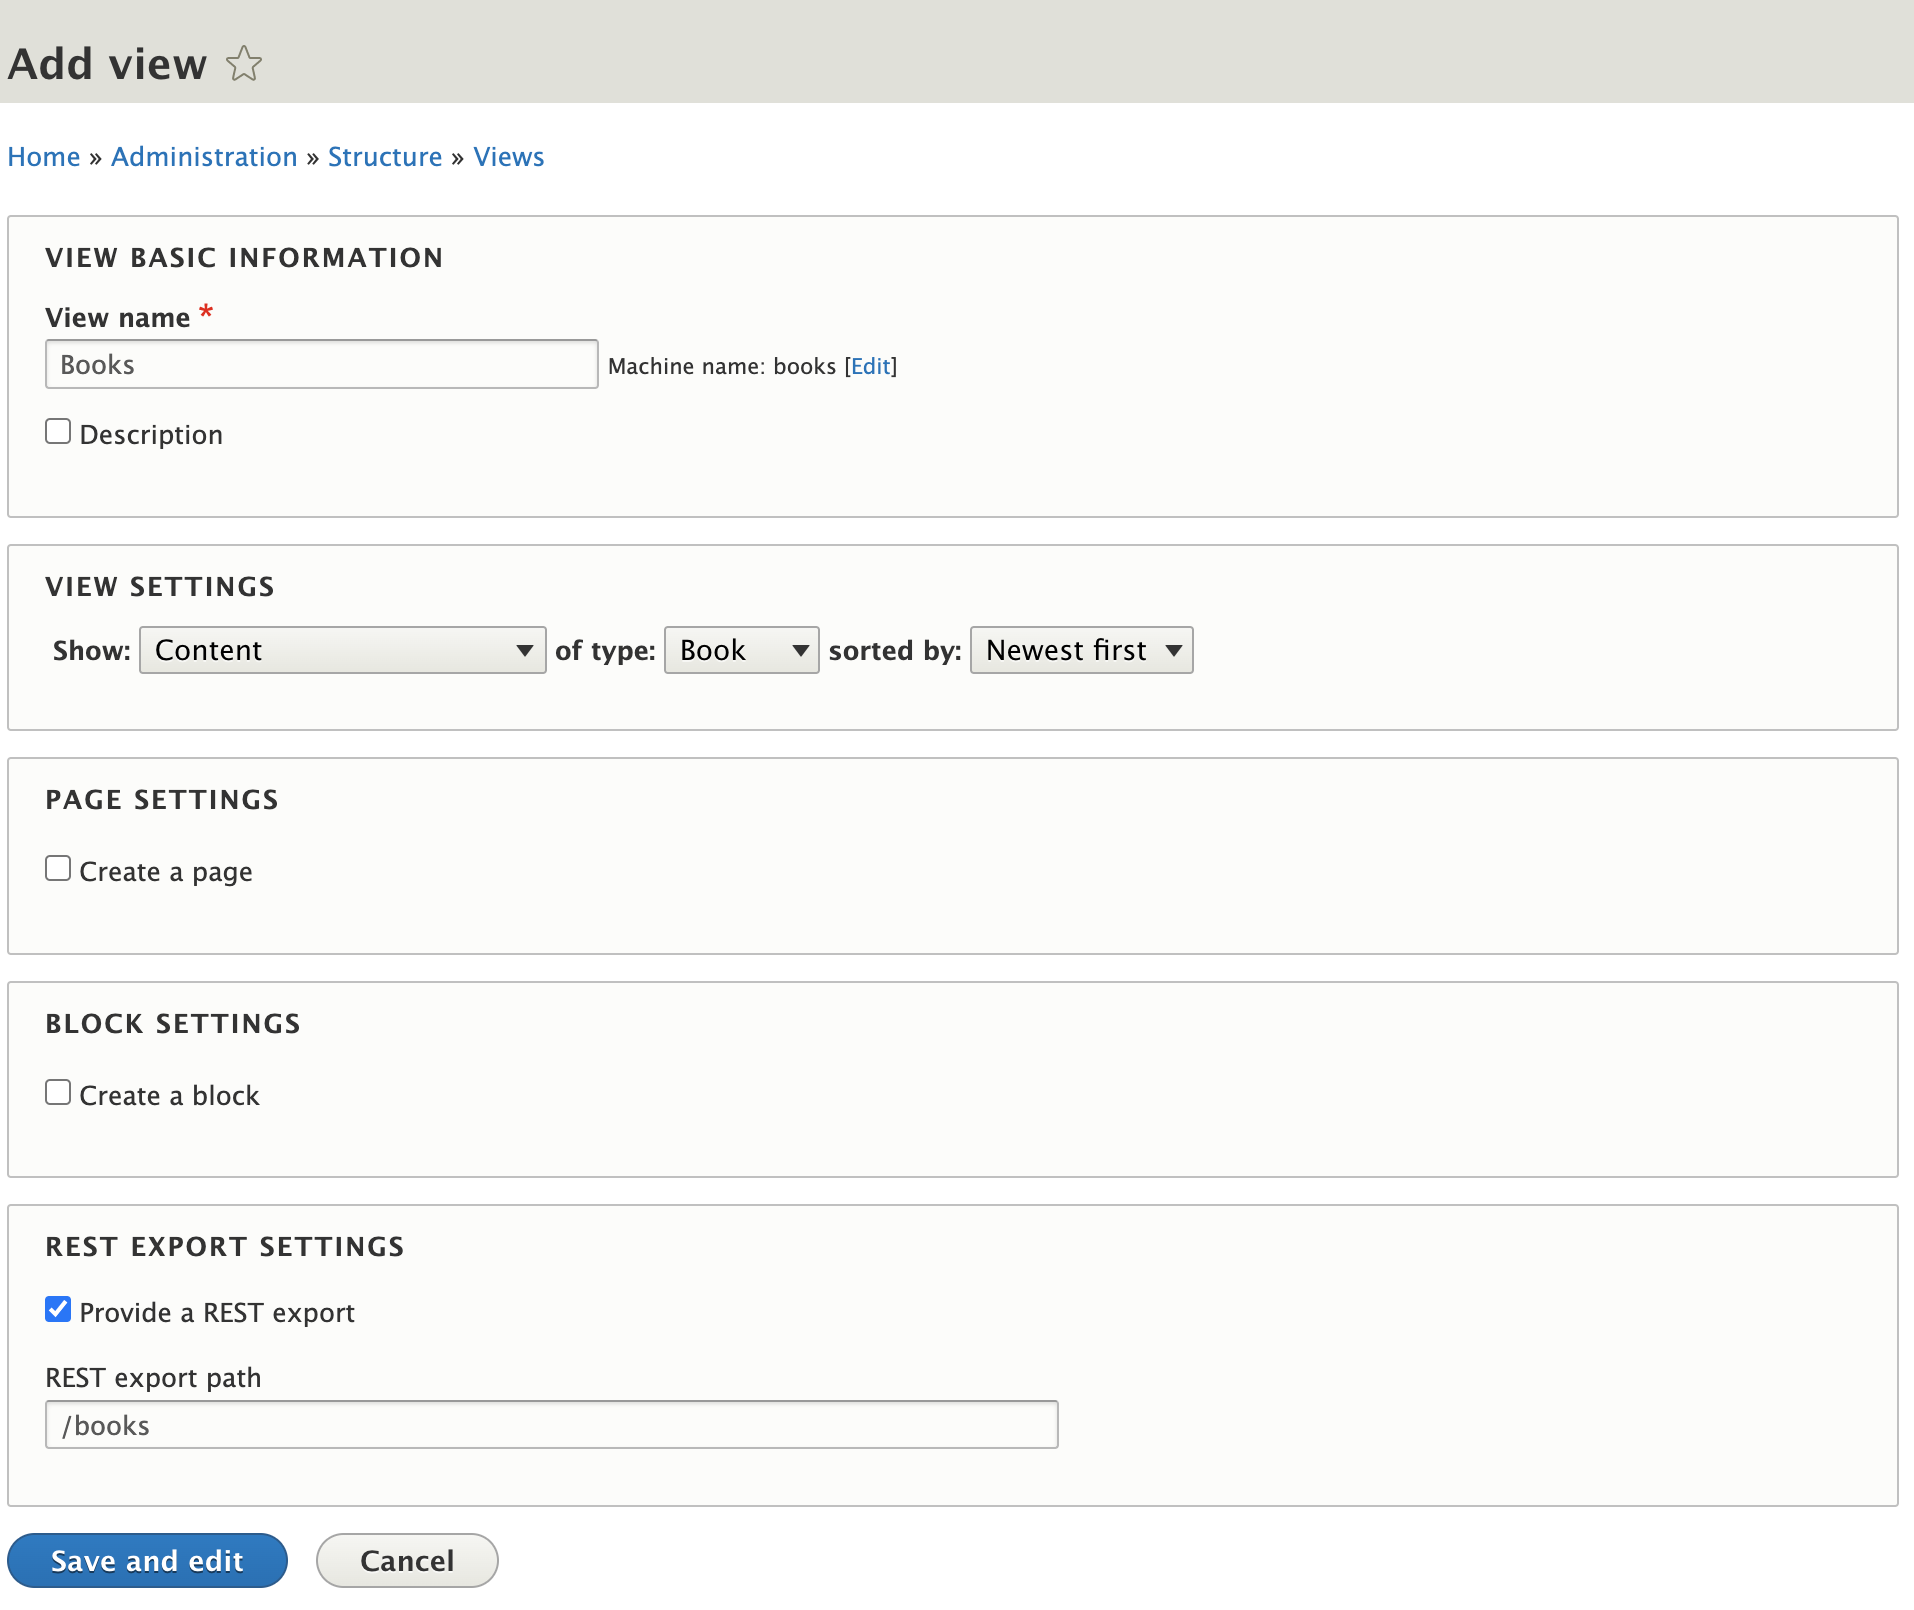
\includegraphics[width=10cm]{./img/View_Create.png}
	\caption[Creating a View]{The configuration page for creating a new view}
\end{figure}

\begin{figure}[h]
	\centering
	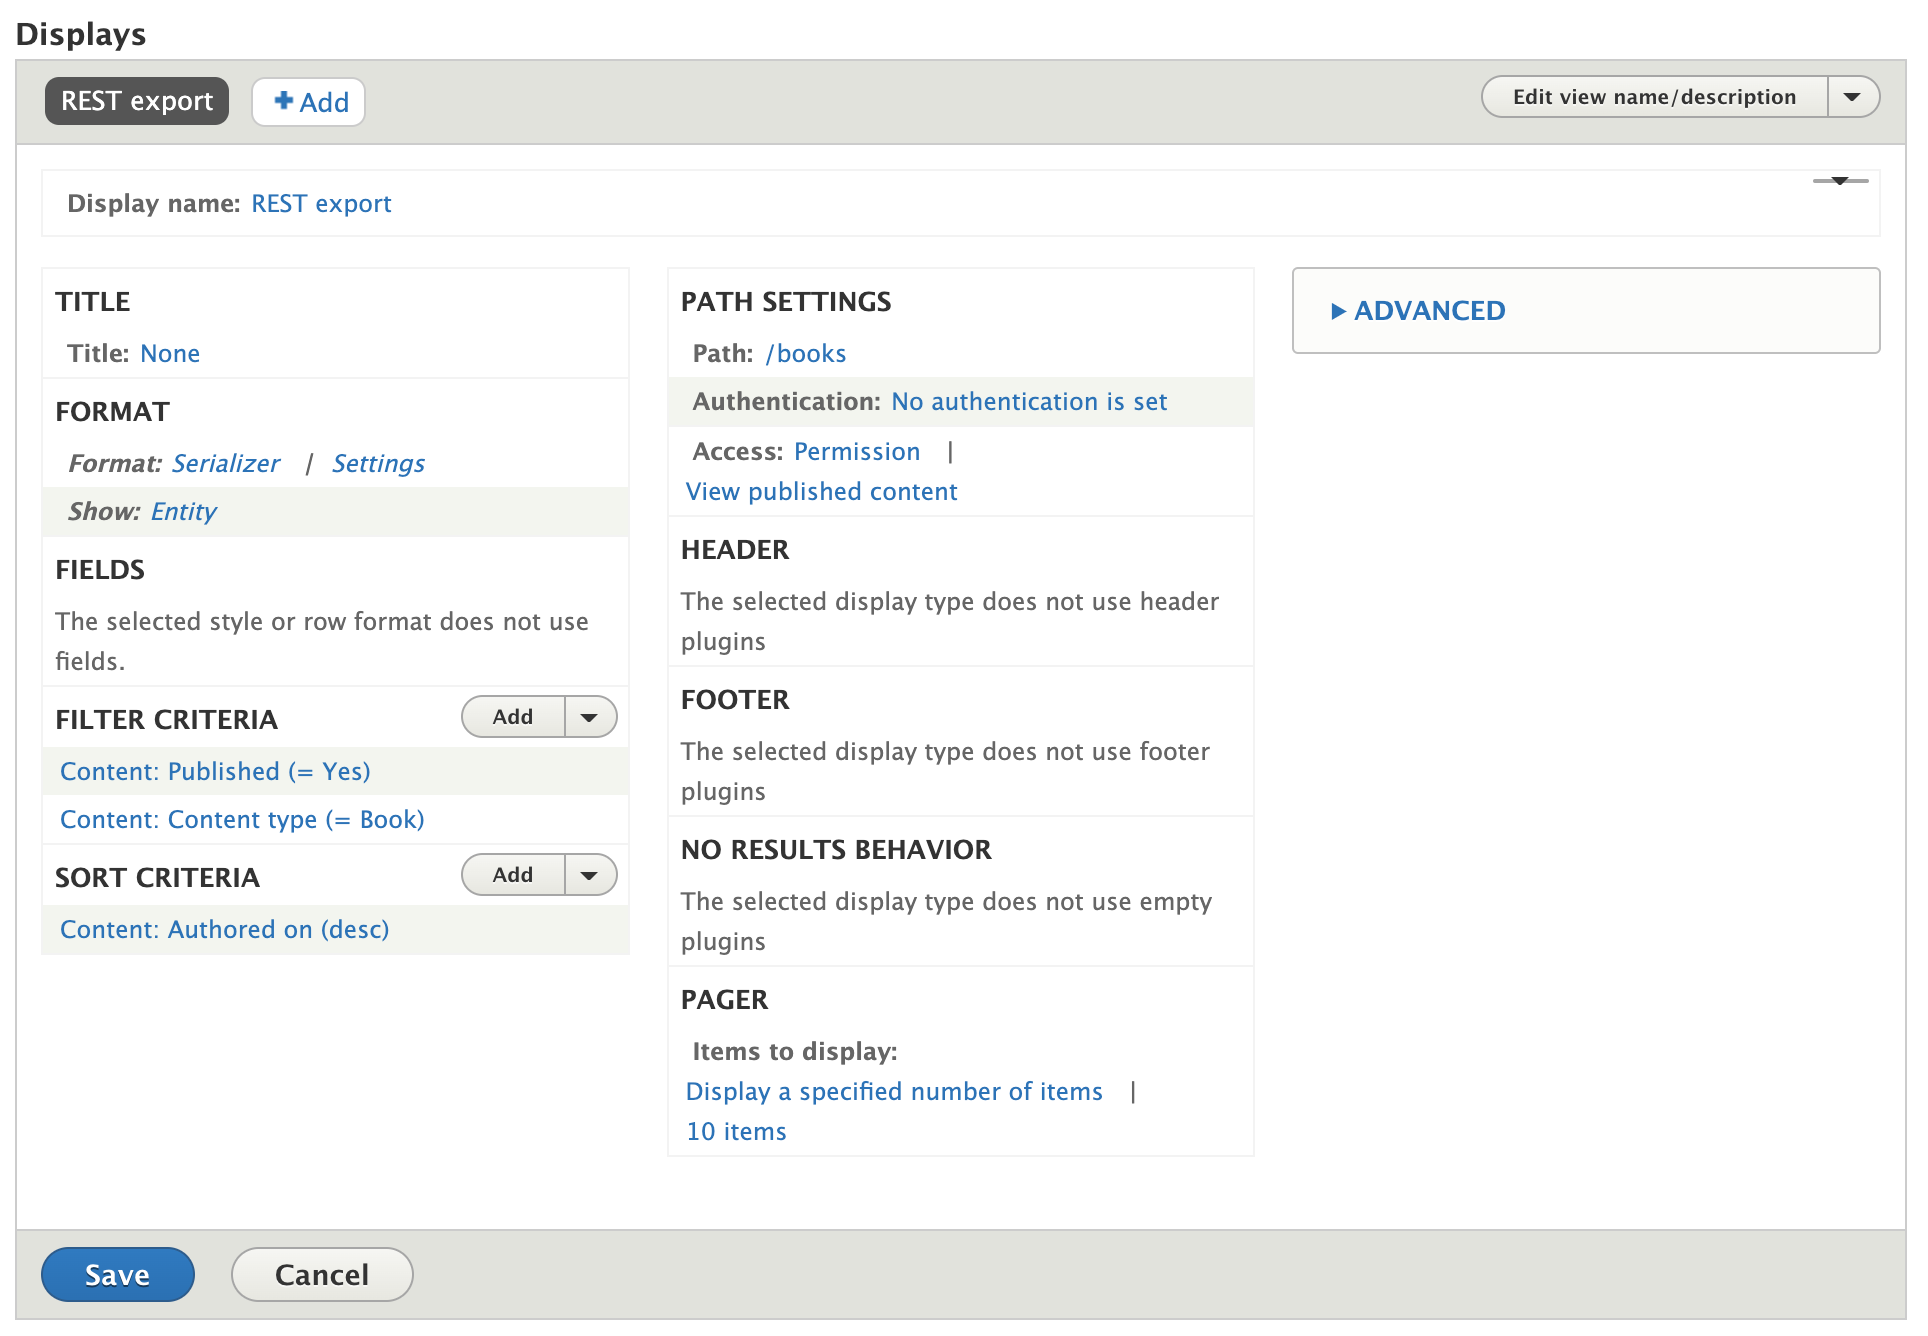
\includegraphics[width=10cm]{./img/View_Details.png}
	\caption[Details of a View]{The details of the newly created view}
\end{figure}

For the purposes of this proof of concept, the output of the JSON:API module will be used to get the data on the front-end, as this module is the one most developers will use, and is the most straight forward to set up.

\section{The front-end}

There are many options to consider on the front-end. These range from the front-end included with Drupal 9, to JavaScript frameworks, to native mobile applications. Basically any framework or tool that has a way to handle HTTP requests through the use of an HTTP client has the possibility to interact with a headless CMS. 

In the following sections the differences between the integrated Drupal front-end and a headless approach will be shown off. Firstly, Drupal Views will be used to display a list of the content that was added previously in the back-end. To show off the headless possibilities, the choice was made to use the front-end JavaScript framework Angular. Angular is an extremely popular framework used around the world to create single page applications. It also has a built-in HTTP client that can be used to create any HTTP request and send it to any domain. This way the data in the Drupal back-end will be displayed.

\subsection{Drupal 9 front-end}

Displaying our data using Views in Drupal is fairly straight forward. As we have already created a view to expose the data using RESTful Web Services, the same view can be used to display the data in Drupal. On the configuration page for the view, a new display can be added by choosing the "Add page" button. 

\begin{figure}[h]
	\centering
	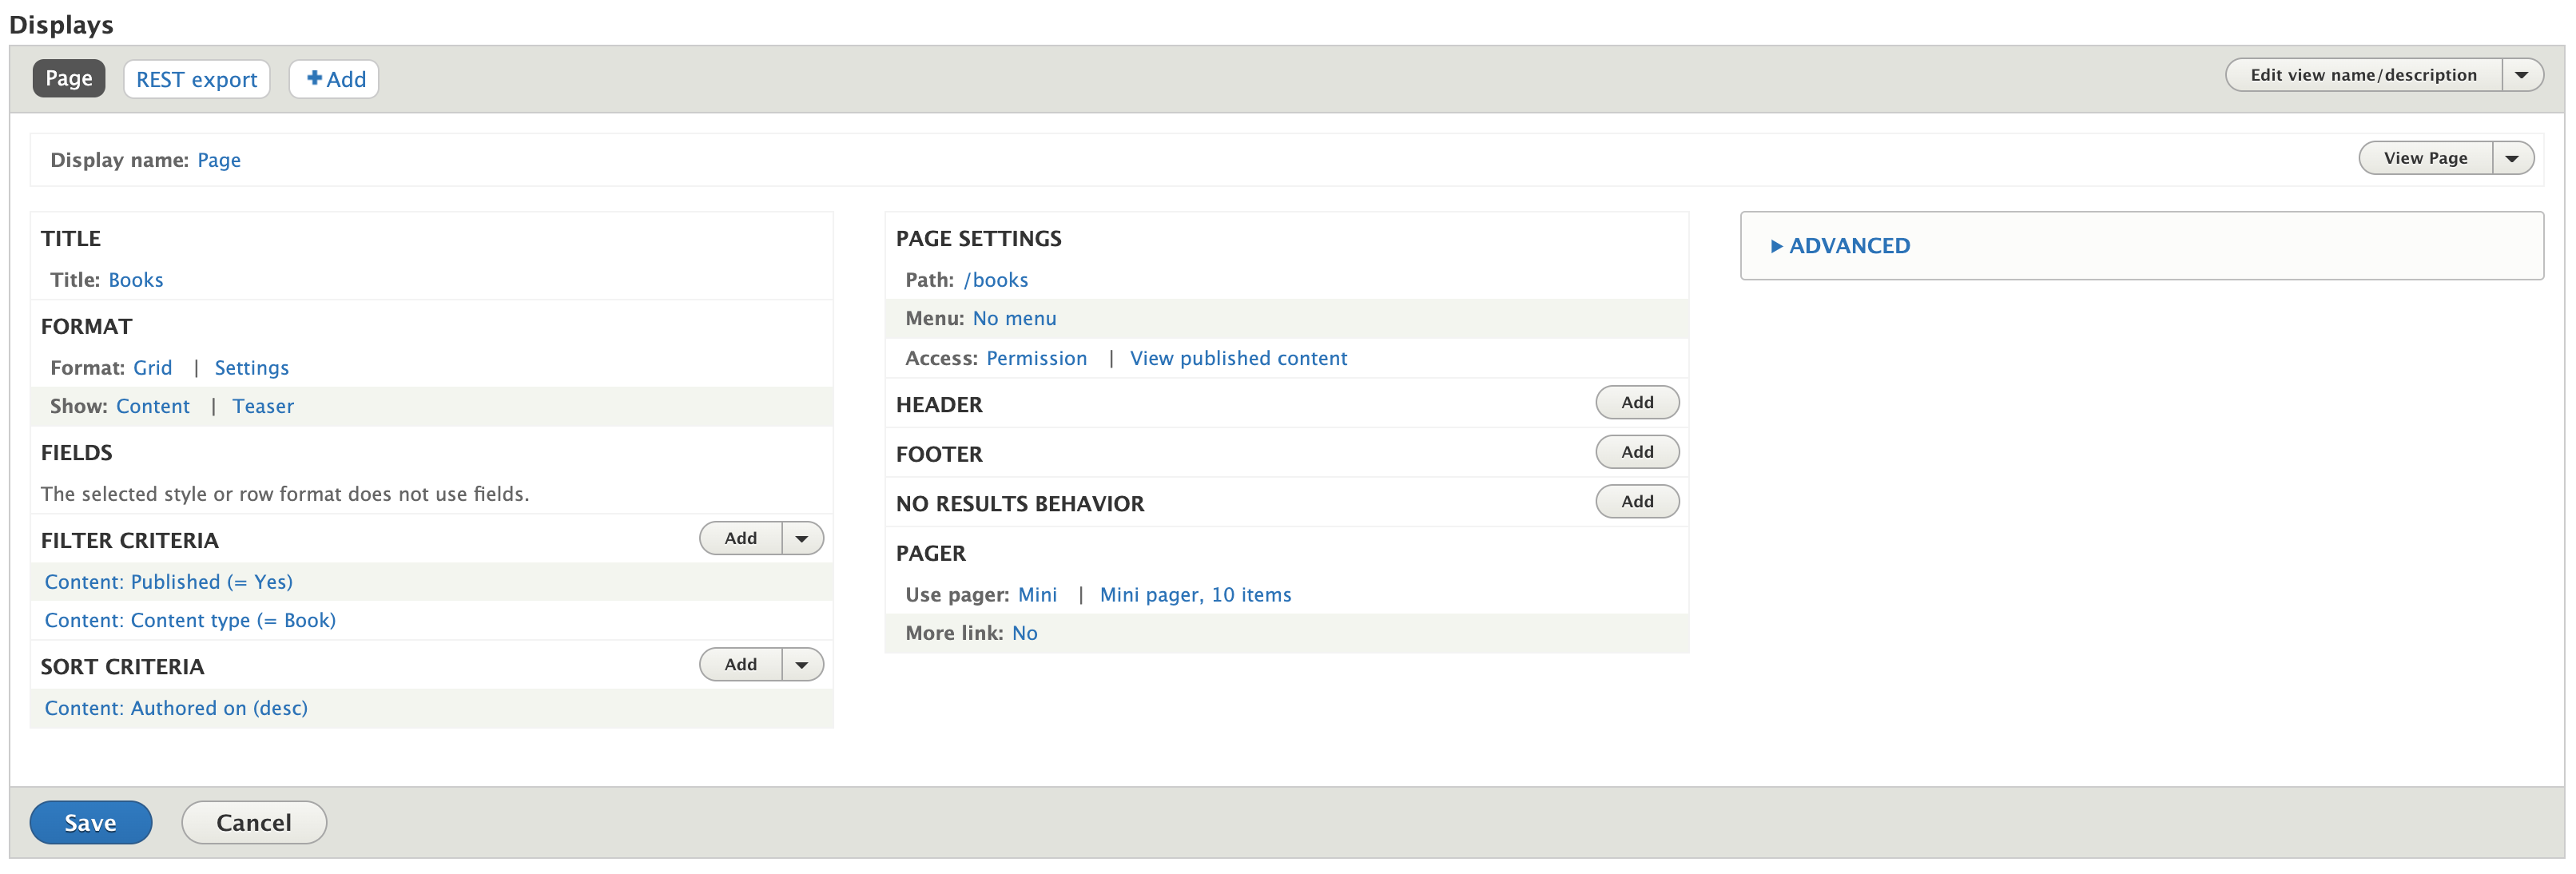
\includegraphics[width=10cm]{./img/Page_View_Config.png}
	\caption[Details of a page display]{The details of a page display}
\end{figure}

This page display can be configured so it shows the content in teaser form. In its default form, this will just contain the title of the book. The teaser of this content type can be configured by going to the content type, and under the "manage display" tab choosing which fields will be displayed for this display. When adding the image, author and abstract fields to this display, the view will use these to display the list of books like in figure \ref{fig:Books}.

As you can see, this is a pretty quick and easy way to be able to display a list of content. Using views, any content can be displayed this way.

\begin{figure}[h]
	\centering
	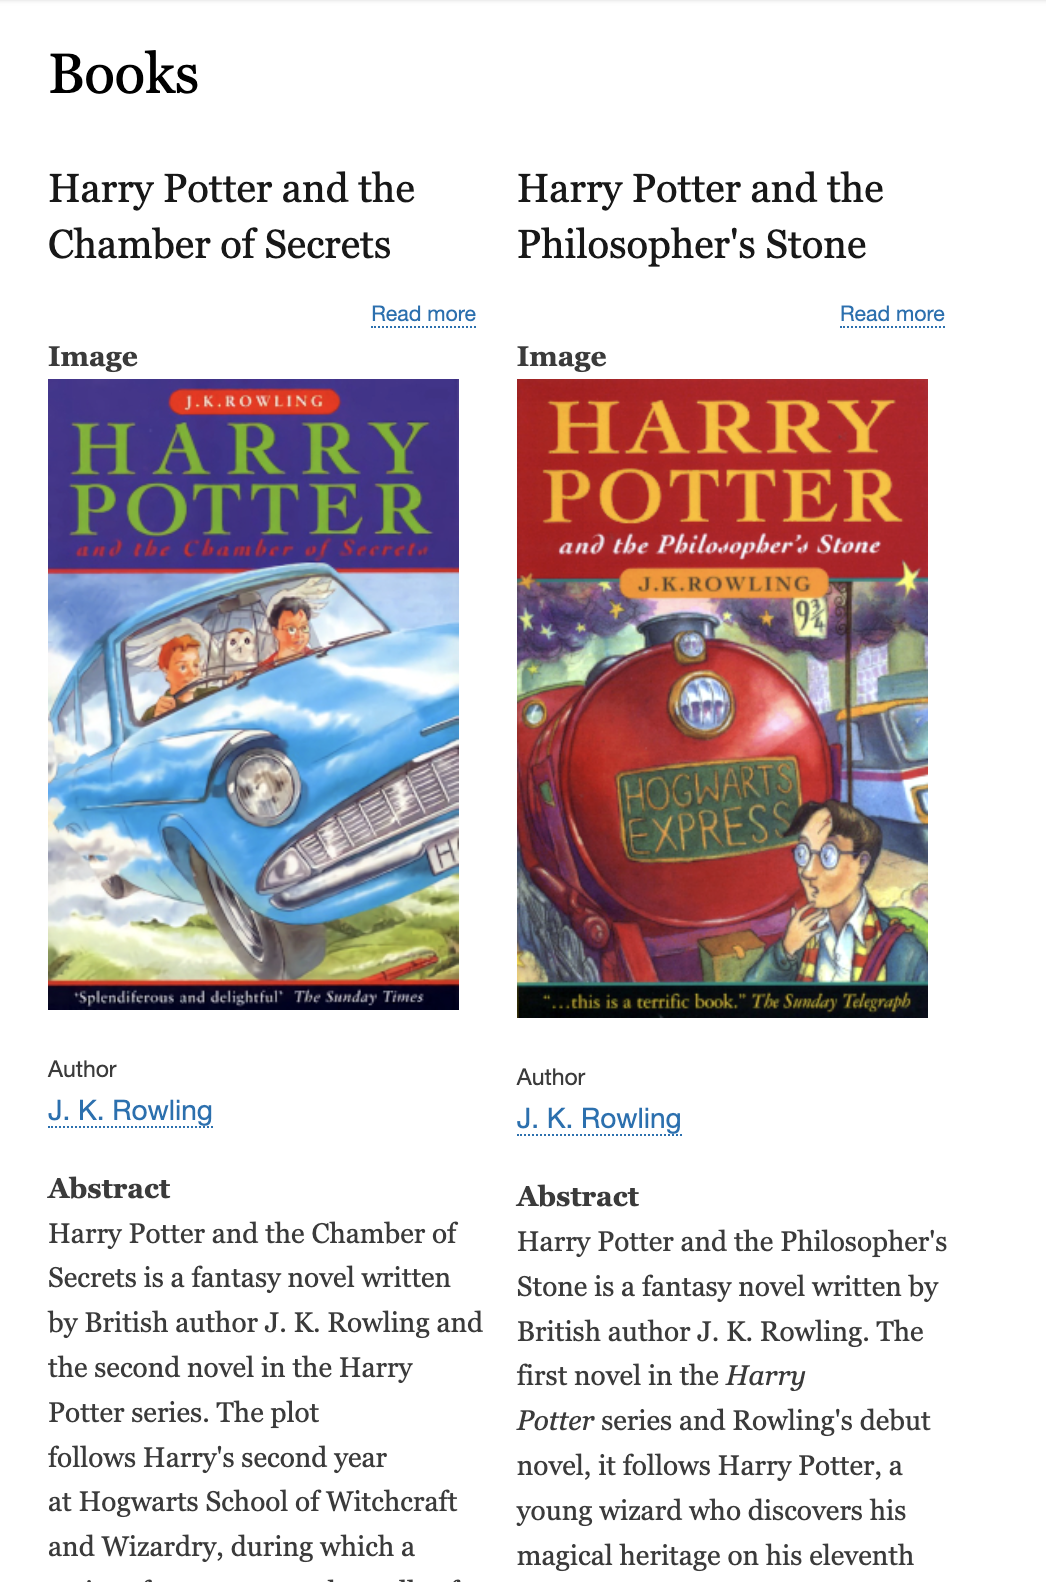
\includegraphics[width=10cm]{./img/Books_Page.png}
	\caption[Display of a list of Books]{The page display of Books displays the fields of all the Books}
	\label{fig:Books}
\end{figure}

\subsection{Single page web application with Angular}

\subsubsection{Preperations and creating a new app}

Creating a new Angular application requires a few differerent things. At the foundation of any JavaScript framework lies \gls{Node.js}. Node.js can be downloaded and installed from \url{https://nodejs.org/en/}. When installing Node.js, \gls{NPM} is usually installed with it. If Node.js is installed, the command "npm install --global @angular/cli@9.0.1" can be used to globally install the Angular CLI, which will be used to make a new Angular project among other things.

To create a new Angular app, you can run "ng new {app-name}", with {app-name} replace by the name of the app. The Angular CLI will then scaffold a new Angular app, meaning that it will create all the necessary folders and files to get started with Angular. With the app created, you can run "ng serve" in the root of the application to start the app.

\begin{figure}[h]
	\centering
	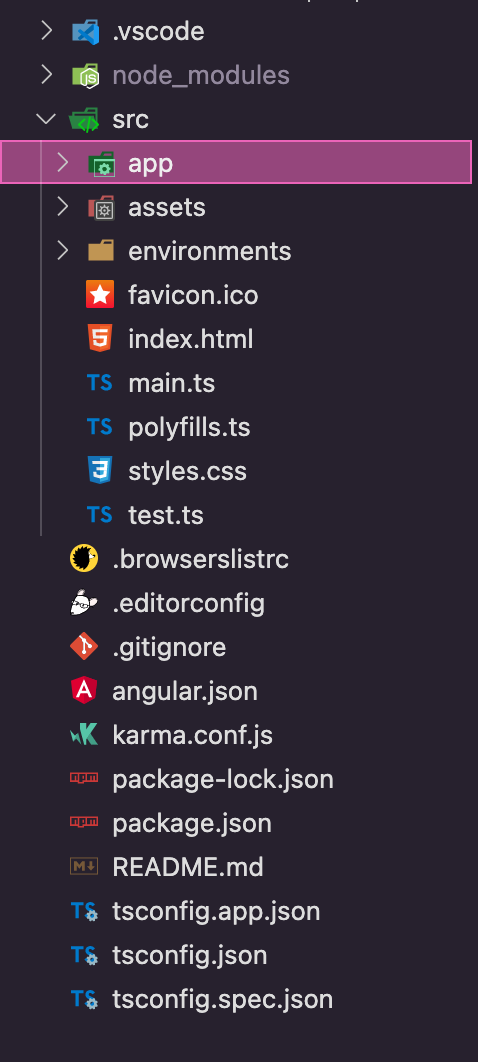
\includegraphics[width=5cm]{./img/Angular_Structure.png}
	\caption[Angular folder structure]{The folder structure of a new Angular application}
\end{figure}

\subsubsection{Creating a new Angular component}

Creating a new component (or building block) can be done by using the Angular CLI. Running "ng new component {component-name}" with {component-name} being replaced by the name of the new component will generate all the files needed. For this example "ng generate component book" is run to create a book component. This component will display a single book. 

As two different components related to books have been created this way, it might be useful to create a book module, which can group these components together. A module can be created by running "ng generate module book --module=app". The "--module=app" option will make sure the module is imported in the app module. 

As the goal is to display a list of books, another component called "Book List" will be required. This can be created by running "ng generate component book-list --module=book". This will generate the files for this component and import it in the new book module. 

\subsubsection{Creating a new Angular service}

Services in Angular are used to accomplish specific tasks. One task a service can perform is to make network requests, so a service will be needed to get the data from the Drupal back-end. This service can be created by running "ng generate service BookService".

To make the connection to the back-end, the Angular HTTP Client will be imported from "@angular/common/http". An instance of this HTTP Client can be injected into the service using dependency injection. When this is done, a get method can be written to GET all the books from the back-end using the JSON:API url: \url{http://localhost:8888/jsonapi/node/book/}. The code for this service looks like this: 


\begin{lstlisting}
	import { Injectable } from '@angular/core';
	import { HttpClient } from '@angular/common/http';
	import { Observable } from 'rxjs';
	
	@Injectable({
		providedIn: 'root'
	})
	export class BookService {
		
		constructor(private _http: HttpClient) { }
		
		get books$() : Observable<any>{
			return this._http.get('http://localhost:8888/jsonapi/node/book/');
		}
	}
\end{lstlisting}

This method will return all the books from the back-end as an Observable, so any component that wishes to have these books can subscribe to this method. In this case, the book-list component will perform this task.

\subsubsection{Subscribing to the service and displaying the data}

To get the data, the book-list-component can subscribe to the method that was just defined in the service. The data that is found within the observable is assigned to a local list that will contain books. The code for this component looks like this:

\begin{lstlisting}
	import { Component, OnInit } from '@angular/core';
	import { BookServiceService } from '../book-service.service';

	@Component({
		selector: 'app-book-list',
		templateUrl: './book-list.component.html',
		styleUrls: ['./book-list.component.css']
	})
	export class BookListComponent implements OnInit {
	
		public books: any;
	
		constructor(private _bookService: BookServiceService) {
			_bookService.books$.subscribe(val => this.books = val.data);
		}
	
		ngOnInit(): void {
	}
	
}
\end{lstlisting}

To display the data that is received a few steps are needed. Firstly,some HTML will be added in the template for the book-list component:
\begin{lstlisting}
<div style="text-align: center;">
	<h1>
		Books:
	</h1>
</div>
<div class="container row">
	<div class="column col-6">
		<div *ngFor="let book of books">
			<app-book [book]="book"></app-book>
		</div>
	</div>
</div>
\end{lstlisting}

Next, the book component will need a field that can contain a single book. This field will be annotated with the @Input() decorator, to indicate that this field will be initialized by each book in the book list.

\begin{lstlisting}
import { Component, Input, OnInit } from '@angular/core';

@Component({
	selector: 'app-book',
	templateUrl: './book.component.html',
	styleUrls: ['./book.component.css']
})
export class BookComponent implements OnInit {
	
	@Input() public book: any;
	
	constructor() { }
	
	ngOnInit(): void {
	}
	
}
\end{lstlisting}

And finally, some more HTML will be added in the template of the book component:




\subsection{Mobile application with SwiftUi}